\documentclass{article}
\usepackage[utf8]{inputenc}
\usepackage{amssymb}
\usepackage{tikz}
\usepackage{amsmath}
\usepackage{relsize}
\usepackage{mathtools}
\usepackage{textcomp}
\usepackage{eurosym}
\usepackage{amssymb}
\usepackage{systeme}
\usepackage{mathtools}
\usepackage{todonotes}
\title{Results}
\author{Roman Oort}
\date{\today}

%%% PERSONAL SHORTCUTS
\DeclareMathOperator*{\plim}{plim}
\newcommand{\T}{\textbf{T}}
\newcommand{\Tij}{\textbf{T}_{ij}}
\newcommand{\Soc}{(\T(n))^{\infty}_{n=1}}
\newcommand{\beli}[3][2]{p_{#2}^{(#3)}}
\newcommand{\belvec}[2]{\textbf{p}^{(#2)}}

\begin{document}

\maketitle

\tableofcontents
\newpage
\section{Results}

All results obtained and discussed in the following section are generated with an identical network structure, unless mentioned otherwise. The networks used are all directed networks, with an increased degree, using the default distribution for the degree increase. Furthermore, the probability of a self-link is $1$, meaning that every agent will have a link to itself. Finally, uniform weight initialization was applied. Furthermore, whenever an updating rule did not lead to uniform convergence, the mean of the belief vector was taken as the convergent belief.

\newpage

\subsection{Cooperative Networks}

As can be seen in Figure \ref{coop:threshold}, the behaviour of a network where the agent update their beliefs using the threshold updating rule is very similar to a network updated through the standard DeGroot mechanics, on all counts. The convergent belief, at nearly every network size, behaves almost identical to the standard DeGroot mechanics. However, where the methods differ most, though so little to be near insignificant, is the standard deviation at the moment of convergence. Where a network converged using standard DeGroot mechanics will converge towards a uniform belief, held by every agent, the belief vector at the time of convergence will have a standard deviation of $0$. On the other, hand when the network is converged using the thresholded updating rule, the convergent belief is not quite uniform, although the difference occurs at the eight decimal point. 

\begin{center}\todo{Fix legend}
    \begin{figure}[!htbp]
        \centering
        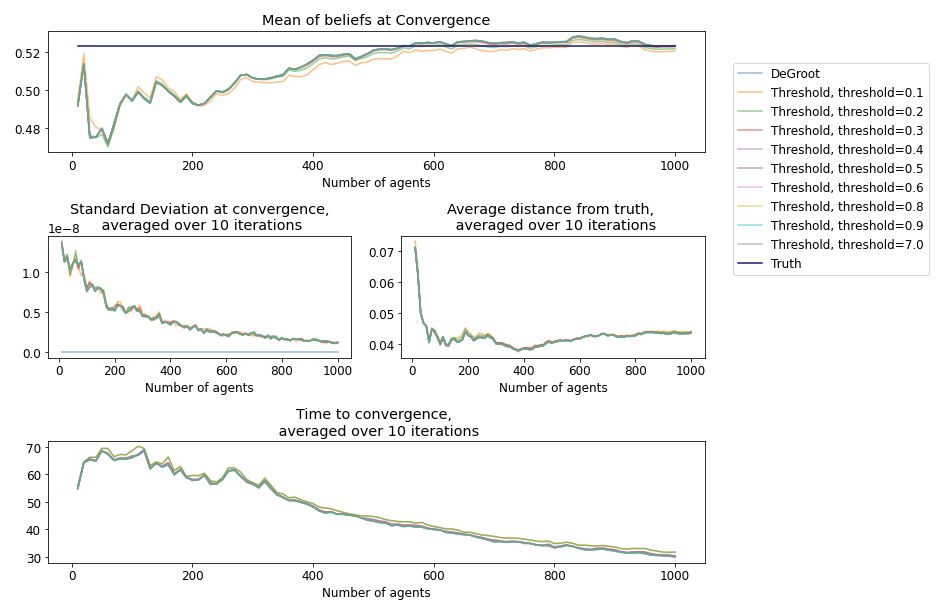
\includegraphics[width=1.2\textwidth]{ThesisKI/Images/WisdomThreshold.png}
        \caption{Convergence Behaviour Threshold Updating}
        \label{coop:threshold}
    \end{figure}
\end{center}

\newpage

However, the private belief rule shows a larger difference between the different parameter values of the updating rules. The convergent belief in the smaller network is seems to differ more for smaller network size, but as the network size increases so too does the similarity between the various values for $\alpha$, the weight placed on the private belief.
Furthermore, as $\alpha$ increases, so too does the standard deviation of the belief vector at the time of convergence, which is to be expected, considering that an increased $\alpha$ will mean that the agents will take more of their initial opinions, which lie the furthest apart from each other, into account when updating. However, the time to convergence does decrease as $\alpha$ increases, as agents' opinions need to change less from their initial opinion when they place more weight on this intial opinion.

\begin{center}
    \begin{figure}[!htbp]
        \centering
        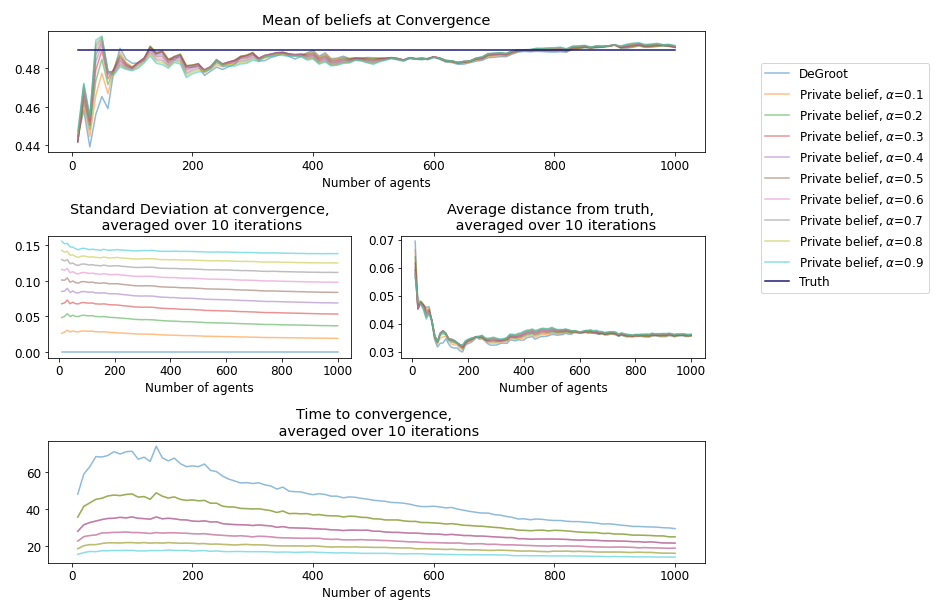
\includegraphics[width=1.2\textwidth]{ThesisKI/Images/WisdomPrivate.png}
        \caption{Convergence Behaviour Private Belief}
        \label{network:noncoop}
    \end{figure}
\end{center}

\newpage

The $\varepsilon$-DeGroot mechanics appear to differ the most from the regular DeGroot mechanics for smaller network sizes. However, similarly to the private belief updating, they tend to behave more and more alike as the network size increases, regardless of the value of $\varepsilon$. However, the standard deviation of the convergent belief vector is considerably higher, though there is a smaller amount of variation dependent on the value $\varepsilon$. Finally, it takes a considerably shorter amount of time to converge a network using $\varepsilon$-DeGroot mechanics rather than the regular DeGroot mechanics. 

\begin{center}
    \begin{figure}[!htbp]
        \centering
        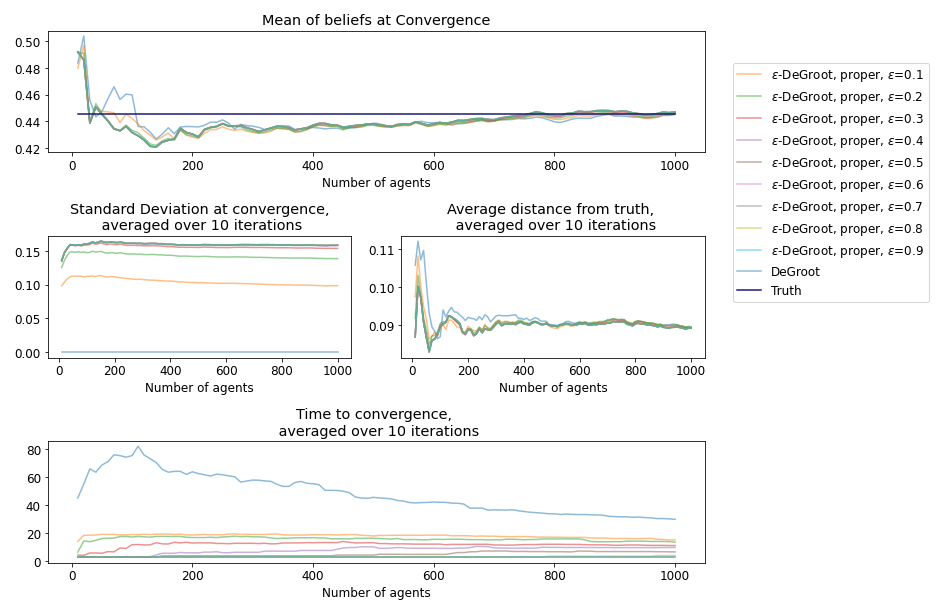
\includegraphics[width=1.2\textwidth]{ThesisKI/Images/WisdomEDeGroot.png}
        \caption{Convergence Behaviour $\varepsilon$-DeGroot}
        \label{network:noncoop}
    \end{figure}
\end{center}

\newpage

Finally, the alternative $\varepsilon$-DeGroot mechanics behave nearly identical to the $\varepsilon$-DeGroot mechanics, though the difference with the regular DeGroot mechanics seems to decrease faster as the network size increases. Furthermore, the non-uniform convergent belief vector remains, just as the faster convergence times.

\begin{center}
    \begin{figure}[!htbp]
        \centering
        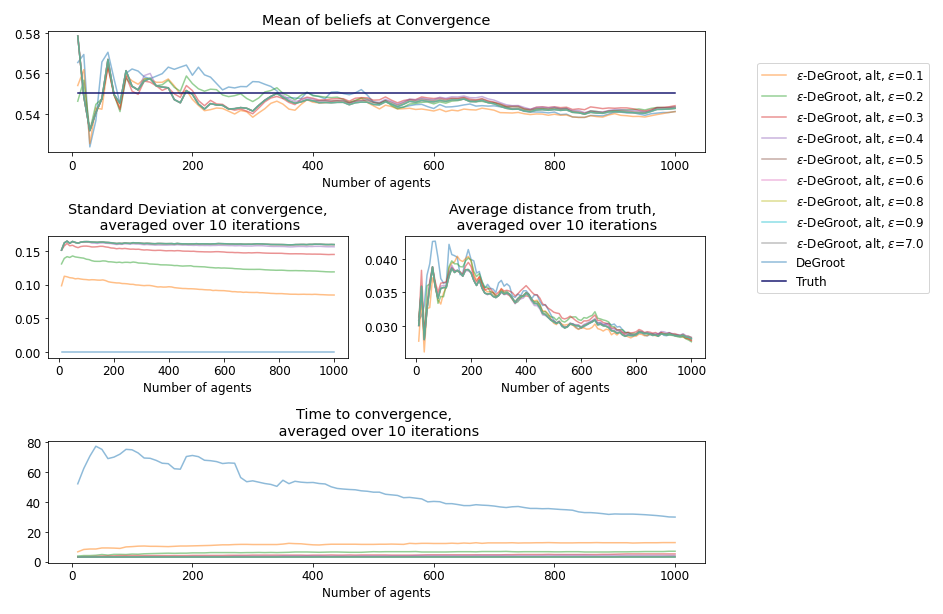
\includegraphics[width=1.2\textwidth]{ThesisKI/Images/WisdomAltEDeGroot.png}
        \caption{Non-cooperative network, $n=50, m=3$}
        \label{network:noncoop}
    \end{figure}
\end{center}




\subsection{Non-cooperative networks, $n=1$}

\subsection{Non-cooperative networks, $n > 1$}

\end{document}